%!TEX root=../Vorlage_DA.tex
%	########################################################
% 				Git
%	########################################################


%	--------------------------------------------------------
% 	Allgmeine Hinweise
%	--------------------------------------------------------
\section{Git}

Git\footnote{\url{https://de.wikipedia.org/wiki/Git}} ist eine dezentrales Versionsverwaltungssystem\footnote{\url{https://de.wikipedia.org/wiki/Versionsverwaltung}} welches urspr\"unglich f\"ur die Entwicklung des Linux-Kernels entwickelt wurde. Es geh\"ort zu den meistgenutzten Systemen in der Open Source Softwareentwicklung, da es gegen\"uber zentralen Versionsverwaltungssystemen diverse Vorteile besitzt:

\begin{itemize}
  \item Kein zentraler Server notwendig
  \subitem Versionshistory ist lokal verf\"ugbar
  \subitem Alle Operationen sind lokal
  \item Kryptographische Sicherheit der Projektgeschichte
%  \item Gute Performance
\end{itemize}

Nachteilig ist, dass es zu Merge-Konflikten kommen kann, wenn mehrere Personen die gleiche Datei ver\"andert haben, und diese von Git nicht automatisch miteinander verschmolzen werden kann. In diesem Fall muss dies manuell durchgef\"uhrt werden. Bei einer Zentralen Versionsverwaltung w\"are dies nicht m\"oglich, da dort nur jeweils 1. Person pro Datei arbeiten darf.

Wir haben uns f\"ur Git entschieden, da wir einerseits durch die Dezentralit\"at gleichzeitig, auch ohne Internetverbindung an dem Projekt arbeiten k\"onnen. Des Weiteren wird uns die M\"oglichkeit gegeben Quellcode\"anderungen mehrerer Personen zu Mergen, sobald eine Funktion ausreichend stabil ist.

\subsection{Grundlegende Funktionsweise}

Bei git besitzt jeder Programmierer ein eigenes Repository, auf welches er \"Anderungen commitet. Diese k\"onnen dann gesammelt auf einen zentrales Repository geladen werden, das dann den aktuellen Projektstand repr\"asentiert.

Wenn ein aktueller Projektstand in das eigene Repository eingecheckt wird, nennt man dies einen Commit. Dieser umfasst die ge\"anderten Dateien, wie auch einen Text welcher die \"Anderungen repr\"asentiert. Lokale Dateien durchlaufen dabei einem grundlegenden Zyklus, in welchen sich der Status der Datei in Relation zum gespeicherten Versionsverwaltungssystem befinden.

\begin{figure}[h]
\centering
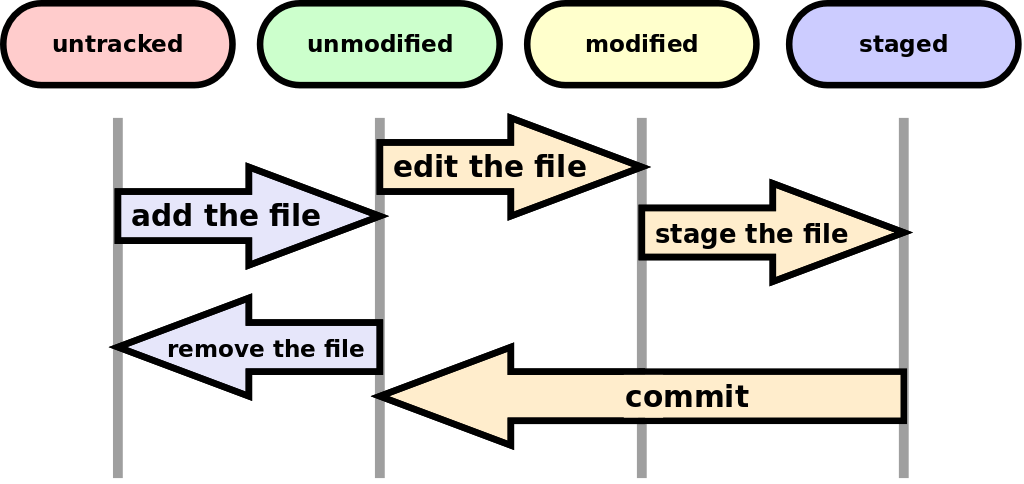
\includegraphics[width=0.9\textwidth]{./media/images/development/git_file_status_livecycle.png}
\caption{grundlegender Zyklus, in der sich der Dateistatus laufend \"andert}
\label{git_file_status_livecycle}
\end{figure}

\htlParagraph{Vormerken aller ge\"anderten Dateien}

\begin{lstlisting}[language=bash]
git add -u
\end{lstlisting}

\htlParagraph{Einchecken  aller Vorgemerkten Dateien}

\begin{lstlisting}[language=bash]
git commit -m 'this is my first commit'
\end{lstlisting}

\newpage

Durch den dezentralen Aufbau besitzt jeder Programmierer zumindest 1 Branch, in welchen commitet wird. Wenn neue Features entwickelt werden kann dies auf einem eigenen Branch geschehen, wodurch das Hauptprojekt bis zum Merge unbeeinflusst weiterentwickelt werden kann. Sobald das Feature fertig ist wird dieses gemergt, und alle \"Anderungen sind so im Hauptzweig vorhanden.

So ist es auch m\"oglich eine Entwicklungsversion wie auch eine Produktivversion als eigenen Branch zu f\"uhren, und so wichtige Patches auf einfache Weise nicht nur in die Entwicklungsversion sondern auch in die Produktivversion anzuwenden, ohne jedoch nicht notwendige \"Anderungen in die Produktivversion zu \"ubernehmen.

\begin{figure}[h]
\centering
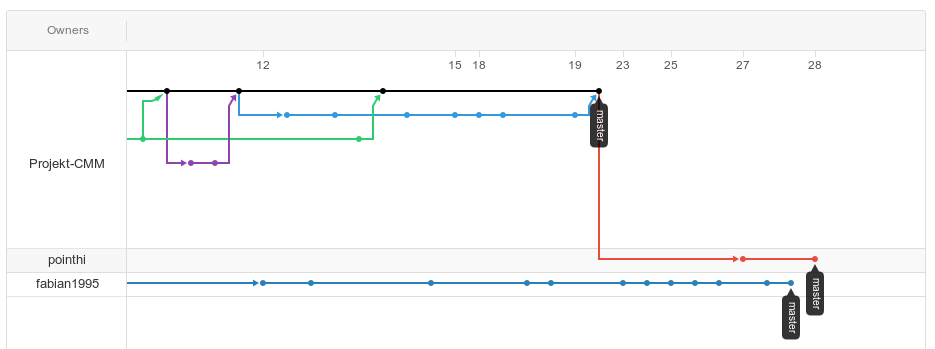
\includegraphics[width=1\textwidth]{./media/images/development/git_history.png}
\caption{Grafische Ansicht des Projektverlaufes, inklusive Branches und  Merges}
\label{development_git_history}
\end{figure}

\section{GitHub}

GitHub\footnote{\url{https://github.com}} ist eine der am weitesten verbreitetsten Hosting-Dienst welcher in der Open-Source Software Entwicklung genutzt wird. Als grundlegende Versionsverwaltung wird git genutzt, welches mithilfe der Webbasierten Oberfl\"ache von GitHub einfach verwaltet wird.

\subsection{Grundlegender Arbeitszyklus}

Wir haben uns auf ein grundlegendes Arbeitsverfahren geeinigt, der sicherstellt dass das Projekt m\"oglichst fehlerfrei verwaltet werden kann. Dazu hat jedes Projektmitglied einen Fork des Projektes auf seinem eigenen GitHub-Repository, mithilfe dessen er dann Pull-Requests an das zentrale Repository stellen kann.

Vorteile dieses Verfahrens sind unter anderem, dass das Mergen im Normalfall auf dem Server geschieht. Des Weiteren wird jedes Pull-Request automatisch getestet, und wird erst nach einem erfolgreichem Test in das zentrale Repository eingecheckt. So werden auftretende Probleme wie fehlende Dateien oder Inkompatibilit\"aten mit anderen \"Anderungen besonders schnell gefunden.